\section{已完成的研究工作及成果}

\subsection{预定计划的执行情况}

目前毕业设计已经收束为以核心算法为中心，围绕控制链、运行时状态和实验验证持续迭代。整体推进大致可分为两个阶段：前一阶段主要集中于 FSM/HITL 骨架、六阶段工作流与工具接入，后一阶段则进一步聚焦于运行时状态、动作选择和横向实验运行基础的补齐。因此，本节对进度的描述不仅反映系统功能是否完成，也反映核心算法是否已经具备相应的系统支撑。

总体而言，当前系统已经完成了从任务接入、候选生成、状态推进、等待态确认、失败恢复到结果汇总的基础闭环，并在此基础上进一步补齐了运行时状态契约、状态快照恢复、动作选择控制流、运行时重排序接口以及横向实验运行器等新内容。系统主体与核心算法主链已经具备较完整的论文支撑基础，但横向对比实验、统一统计图表和工作量定量汇总尚未完全收口。

\begin{table}[htbp]
	\centering
	\caption{项目进度及毕业设计（论文）工作计划完成情况表}
	\label{tab:midterm-plan-progress}
	\renewcommand{\arraystretch}{1.22}
	\fontsize{9.2pt}{12.8pt}\selectfont
	\begin{tabularx}{\textwidth}{p{2.1cm}p{2.1cm}>{\raggedright\arraybackslash}X p{2.5cm}}
		\toprule
		起始时间 & 完成时间 & 计划工作内容 & 备注（是否已完成） \\
		\midrule
		2025.12.26 & 2026.01.15 & 完成 FSM/HITL 重构、PendingAction/Decision/TaskSnapshot/EventLog 等核心对象设计，建立任务状态推进、人工决策与审计记录的基本框架。 & 已完成 \\
		2026.01.14 & 2026.01.25 & 完成 ProteinToolKG 最小可用形态与从头蛋白质设计最小闭环，初步形成“规划、执行、失败判定、结果汇总”的连续链路。 & 已完成 \\
		2026.02.01 & 2026.03.08 & 完成系统演示链路与工具扩展，补齐任务状态展示、PendingAction 决策界面、事件时间线及远程工具接入能力。 & 已完成 \\
		2026.03.01 & 2026.03.15 & 完成 CandidateSet v1、Top-K 候选生成、风险与成本门禁、六阶段工作流关键能力以及中期实验冻结与治理复核基础。 & 已完成 \\
		2026.03.16 & 2026.03.23 & 完成基线冻结、证据目录冻结、全流程验证矩阵、远程 REST 端到端验证和高代价实验指标补充，为后续算法对照提供统一基线。 & 已完成 \\
		2026.03.24 & 2026.04.03 & 完成运行时状态契约冻结、状态快照恢复、候选与等待态运行时摘要、决策与恢复链审计字段补充。 & 已完成 \\
		2026.04.01 & 2026.04.10 & 完成 Lite belief-state 更新主链、运行时影子重排序接口、自适应动作选择控制流及 \texttt{terminal\_stop} 语义映射。 & 已完成 \\
		2026.04.08 & 2026.04.21 & 完成多工具统一验收接口、纵向实验运行器扩展、横向实验运行器与部分真实结果沉淀，形成新一轮方法迭代基础。 & 阶段性完成 \\
		2026.04.01 & --- & 横向对比实验结果收口、统一图表统计、工作量定量汇总和论文文字收束仍需继续推进。 & 进行中 \\
		\bottomrule
	\end{tabularx}
\end{table}

\normalsize
由表 \ref{tab:midterm-plan-progress} 可见，项目已经完成了从基础控制面到运行时算法增强的连续迭代。当前工作的重点已经从单纯的系统骨架搭建，转向围绕核心算法所需的运行时状态建模、动作选择和对照实验基础展开。

\subsection{核心算法设计与阶段性完成情况}

本阶段在原有 FSM、HITL 和恢复框架之上，将研究主线明确收束为面向高代价蛋白质设计工作流的自适应工具链规划算法。依据当前设计目录中的 \texttt{core-algorithm-spec}，该算法研究的不是简单的 ToolKG 检索，也不是从少量工具中静态选出一条路径，而是要回答：在高代价、长链路、可失败、可恢复的工作流中，系统如何动态生成、评估、裁剪并修正候选工具链，以降低无效高代价调用并提高整体任务成功率。

从问题形式上看，该算法的输入包括设计目标、结构化约束、工具能力图、当前执行上下文以及运行时观测；输出则不是单条固定工具链，而是当前候选工具链集合、默认推荐候选，以及在必要时给出的局部修补、后缀重规划或终止建议。由此，算法所处理的是一个同时具有约束感知、预算感知、风险感知和恢复感知特征的工作流级动态规划问题，而不是单步工具选择问题。

从候选语义上看，算法在关键控制点显式维护三类结构化候选：初始规划对应 \texttt{PlanCandidate}，局部修补对应 \texttt{PatchCandidate}，后续替换对应 \texttt{ReplanCandidate}。每个候选不仅需要给出可执行的结构化载荷，还需要同时附带 \texttt{score\_breakdown}、\texttt{risk\_level}、\texttt{cost\_estimate} 和解释信息，从而使候选比较不再停留在模糊的“哪个好”判断上，而是可以围绕可执行性、目标贴合度、风险、成本和恢复复杂度展开统一比较。在这一框架下，\texttt{stop} 并不被视为普通异常，而是作为一种终止型重规划语义存在，即当前剩余后缀被判定为不值得继续投入，但已验证前缀仍然作为可审计资产保留。

从优化目标上看，算法并不试图单独最大化某一条候选链的先验得分，而是追求更高任务成功率、更少无效高代价调用、更低恢复复杂度以及更合理的人机分工。换言之，静态评分阶段不仅要考虑目标达成度，还要显式考虑成本惩罚、风险惩罚和恢复复杂度惩罚；运行时阶段则进一步结合新的观测，决定当前候选是否仍值得继续执行。这样的目标设置使得系统在面对高代价步骤时能够更保守地控制资源投入，而不是在单次规划后盲目执行到底。

从当前设计与方法结构来看，该算法已经形成较清晰的三层结构。第一层是静态候选规划层，负责根据任务目标、结构化约束、工具能力图与治理策略生成 \texttt{PlanCandidate}、\texttt{PatchCandidate} 和 \texttt{ReplanCandidate} 等 Top-K 结构化候选，并通过可执行性、目标贴合度、风险、成本和恢复复杂度进行静态多目标评分。第二层是运行时自适应层，负责从 \texttt{StepResult}、\texttt{SafetyResult}、恢复历史、预算使用情况和等待态摘要中提取运行时观测，更新轻量运行时状态，并通过 \texttt{runtime reranking} 对已通过静态校验的候选做再次排序。第三层是动作选择层，负责在不破坏 FSM 合法迁移、Agent 职责边界以及 \texttt{retry -> patch -> replan} 恢复顺序的前提下，对当前链路给出 \texttt{continue}、\texttt{patch\_local}、\texttt{suffix\_replan} 或 \texttt{stop} 等治理动作建议。

其中，运行时状态并不被设计为新的控制器或新的 Agent，而是作为算法内部的轻量状态估计模块存在，用于承载成功概率、结构性失败倾向、恢复余量、剩余成本暴露和证据充分性等关键信息。它的作用不是替代静态评分，而是通过 \texttt{runtime reranking} 对已经通过静态可执行性校验的候选进行有界修正，从而回答“这条链路在当前已经运行到这里时是否仍值得继续”的问题。相应地，动作选择层也不是任意开放的决策器，而是严格受制于现有状态机、恢复顺序和人工确认约束，只在允许的治理动作空间内做出选择。

\begin{figure}[htbp]
	\centering
	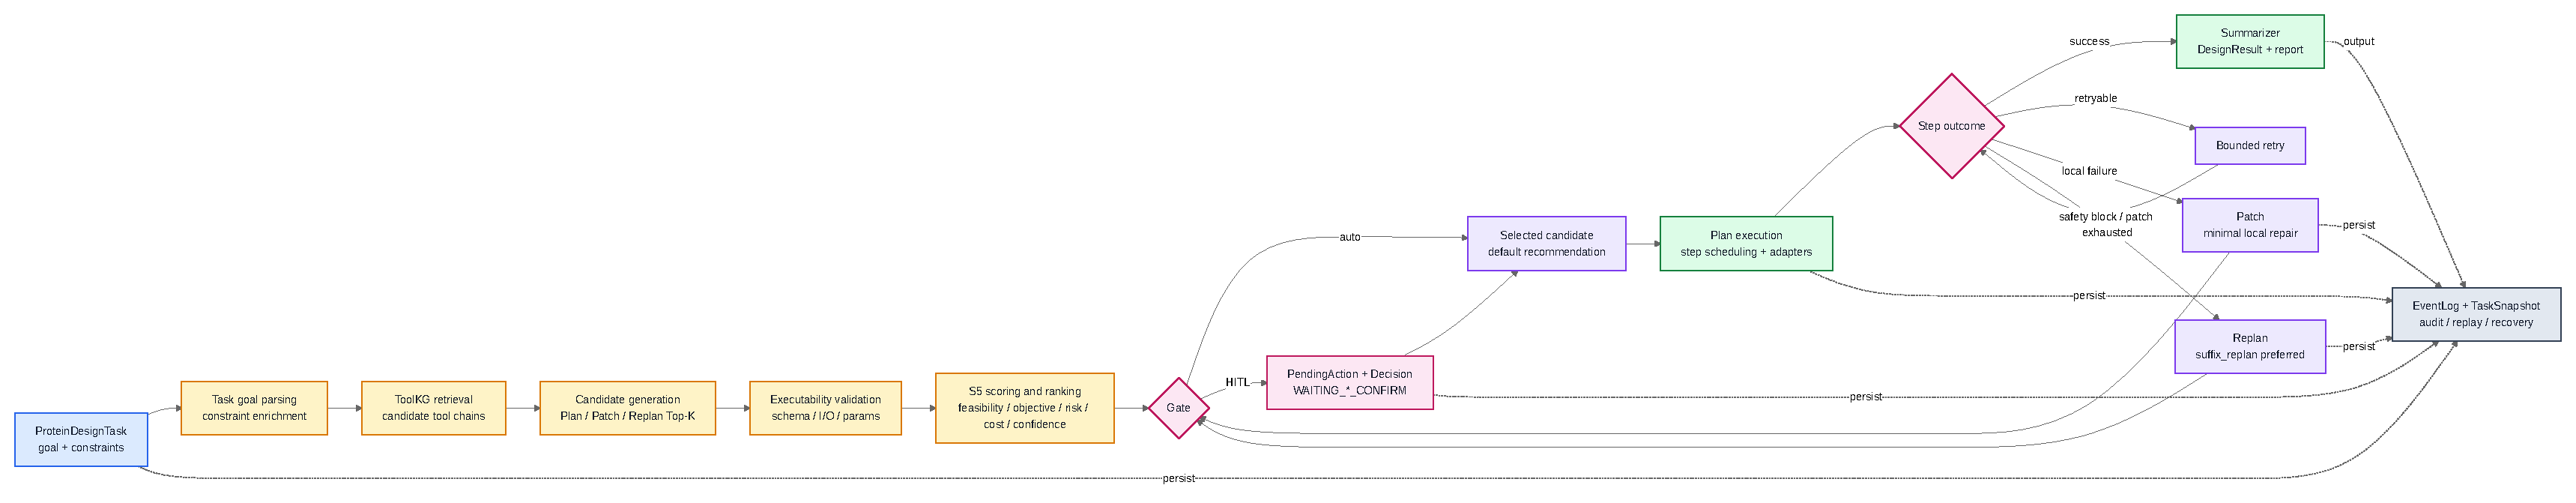
\includegraphics[width=0.95\textwidth]{../figures/core-algorithm-overview.pdf}
	\caption{核心算法总体结构示意图}
	\label{fig:midterm-core-algorithm}
\end{figure}

如图 \ref{fig:midterm-core-algorithm} 所示，算法主线已经能够被明确划分为候选工具链生成、静态评分、运行时状态更新和动作选择四个连续阶段。图中尤其强调，运行时部分并不是对静态评分的简单附加，而是通过对工作流执行状态的持续估计，对候选链路进行再次判断，并在必要时触发局部修补、后缀重规划或终止止损。这一结构使算法从“候选排序器”进一步提升为“工作流级动态规划器”。

\begin{table}[htbp]
	\centering
	\caption{核心算法三层结构及当前完成情况}
	\label{tab:midterm-algorithm-layers}
	\renewcommand{\arraystretch}{1.22}
	\begin{tabularx}{\textwidth}{p{2.8cm}p{4.0cm}>{\raggedright\arraybackslash}X p{2.0cm}}
		\toprule
		算法层次 & 主要输入 & 主要输出/职责 & 当前状态 \\
		\midrule
		静态候选规划层 & 任务目标、约束、ToolKG、策略配置 & 生成 \texttt{Plan/Patch/Replan} 候选集，完成静态可执行性校验与多目标评分 & 已完成 \\
		运行时自适应层 & \texttt{StepResult}、\texttt{SafetyResult}、恢复历史、预算使用、等待态摘要 & 更新 Lite runtime state，并通过 \texttt{runtime reranking} 修正候选优先级 & 已完成 \\
		动作选择层 & 静态评分、运行时状态、策略约束、恢复上下文 & 在 \texttt{continue / patch\_local / suffix\_replan / stop} 之间做出治理动作建议 & 已完成 \\
		\bottomrule
	\end{tabularx}
\end{table}

如表 \ref{tab:midterm-algorithm-layers} 所示，本文算法的关键组成已经全部具有明确的输入、输出与系统落点。FSM、HITL、恢复链和六阶段工作流并不是与算法平行存在的若干工程模块，而是该算法在真实场景中的运行约束与观测来源。也就是说，系统工程的意义在于为算法提供可运行、可观测、可审计的实验平台，而不是替代算法本身。

需要进一步说明的是，本文在这一部分强调的是核心算法的定义、输入输出、目标与动作语义，而不是具体实现过程。当前版本并未将研究目标扩展为完整的学习型控制器或完整 POMDP 求解，而是采用了更适合当前阶段的 Lite 版本：在保持现有 FSM、HITL 和恢复闭环稳定的前提下，把运行时状态估计作为自适应规划算法的内部模块引入，使其与候选排序、动作选择和恢复控制形成耦合。这样的边界既保证了方法的算法性和独立性，也避免了把研究范围扩张到难以在毕设周期内完成的程度。

\subsection{系统总体设计与实现进展}

在系统层面，当前实现已经形成“算法层嵌入运行时骨架”的较稳定结构。任务从接口层进入后，首先被统一封装为任务对象；随后，Planner 结合 ToolKG 产生候选集并输出静态评分；Workflow Runtime 在候选门禁、等待态固化和状态推进上承担控制职责；Executor 负责执行、失败检测与恢复触发；Safety 和 Summarizer 分别提供风险判断和结果整理；事件日志与任务快照则负责为运行时状态、动作应用和实验分析提供证据沉淀。这一结构保证核心算法增强并没有破坏既有系统，而是以内聚方式与现有控制面融合。

\begin{figure}[htbp]
	\centering
	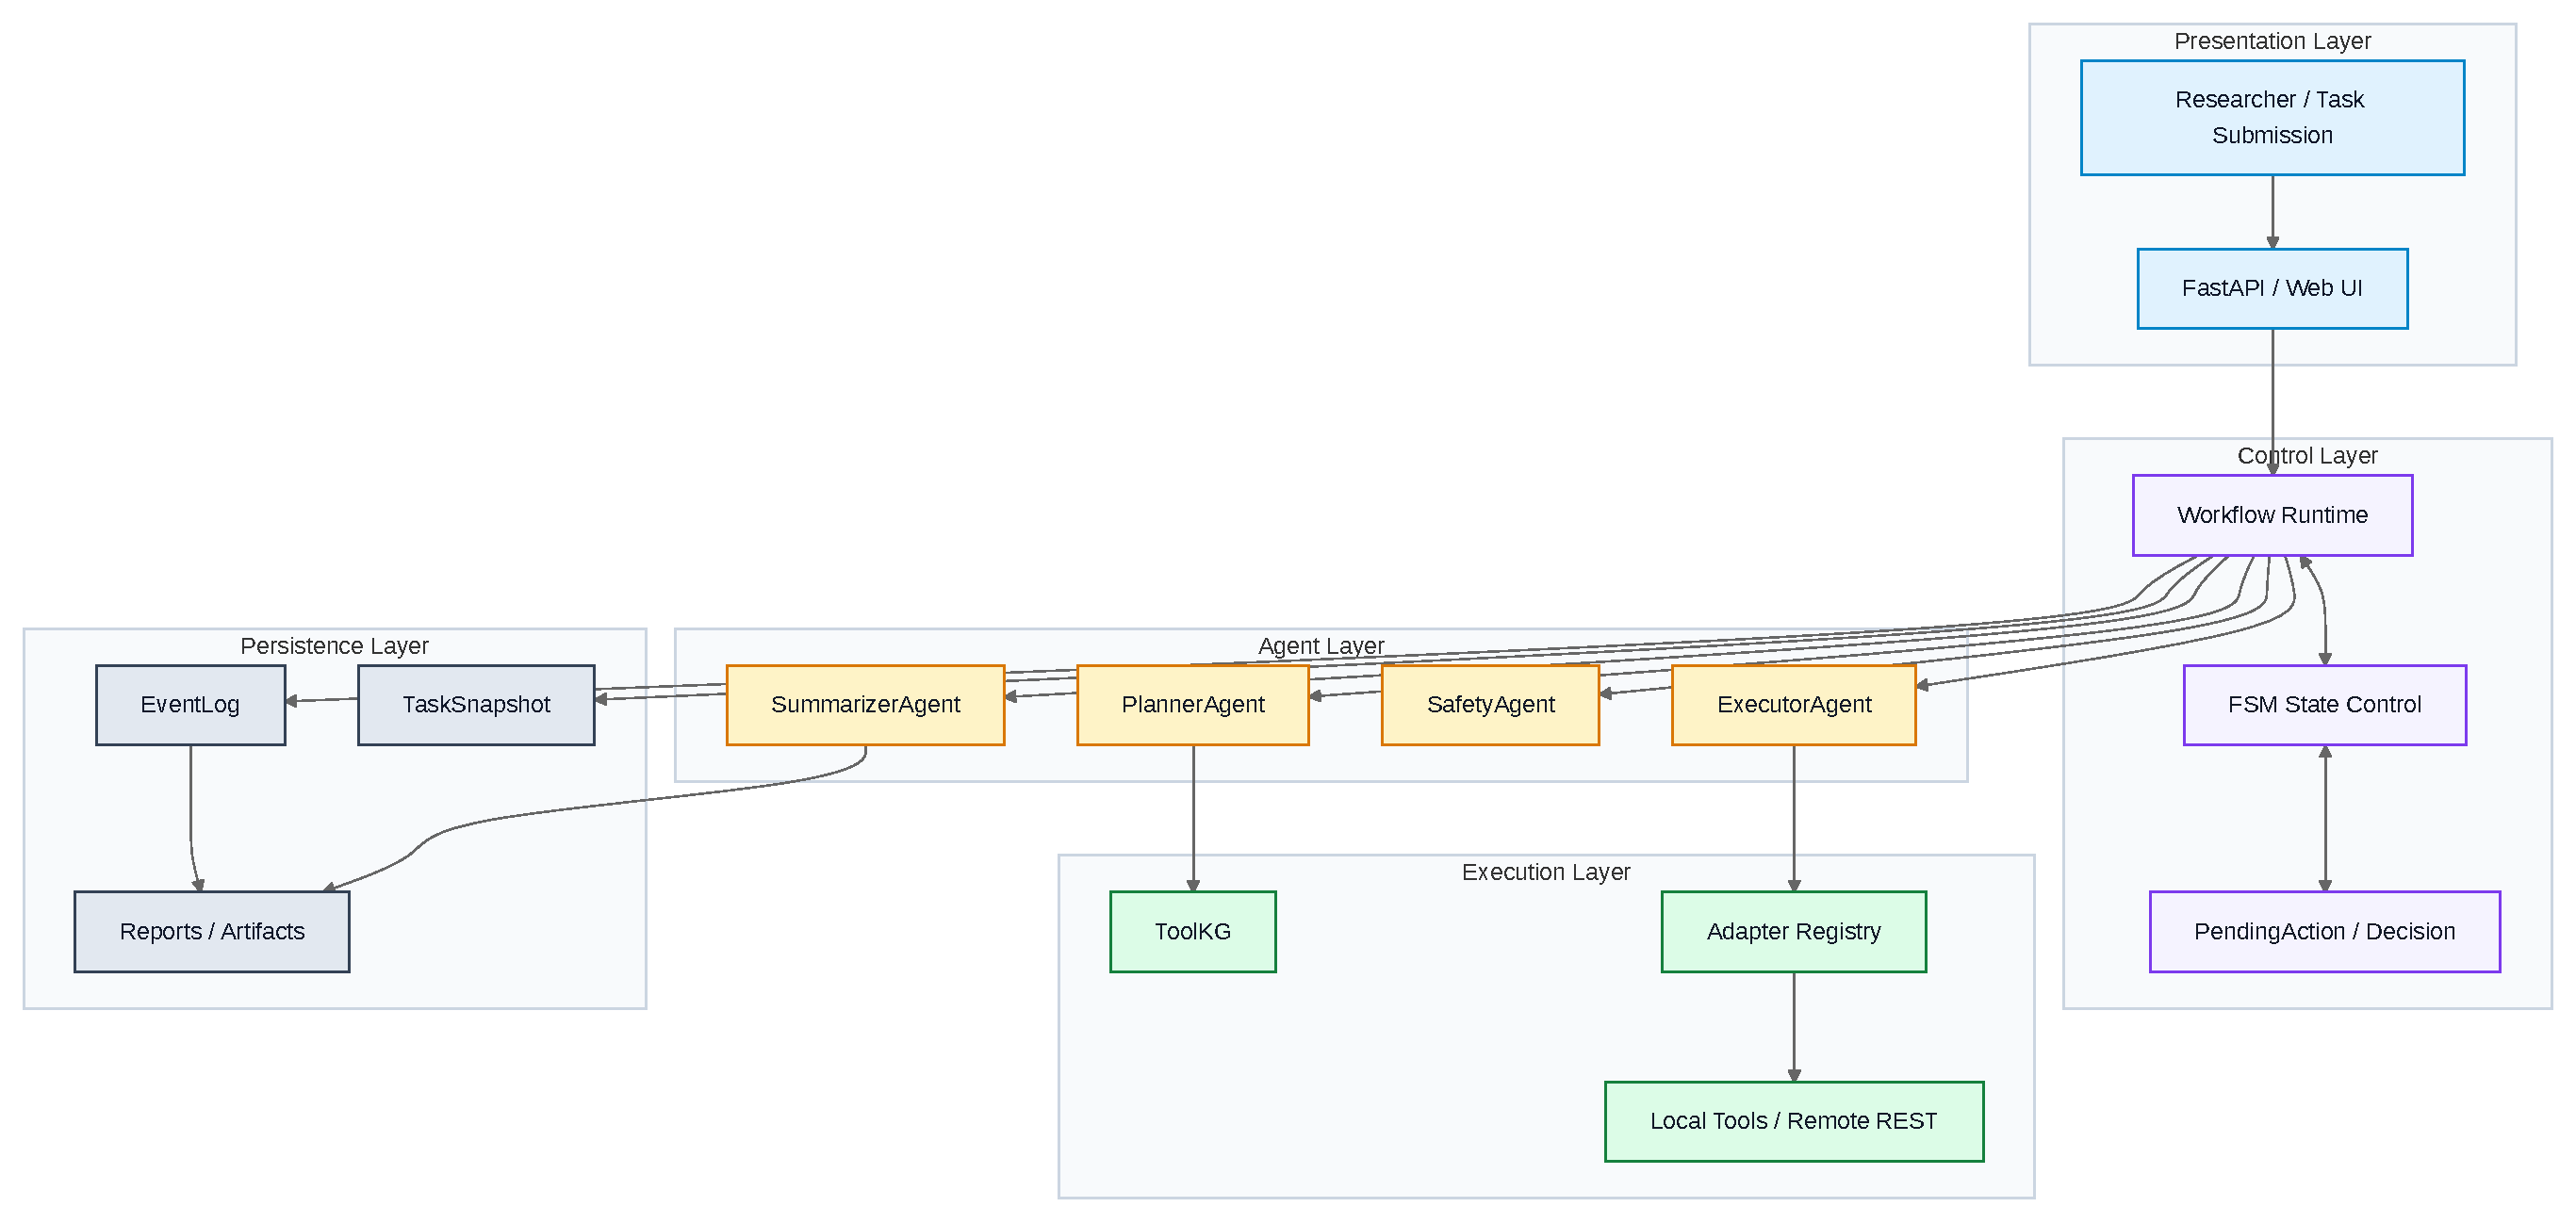
\includegraphics[width=0.95\textwidth]{../figures/system-architecture-overview.pdf}
	\caption{系统分层架构与算法嵌入位置}
	\label{fig:midterm-architecture-overview}
\end{figure}

如图 \ref{fig:midterm-architecture-overview} 所示，系统整体仍沿输入层、规划与控制层、执行与恢复层、安全与汇总层以及资源层展开，但与早期版本不同的是，规划与控制层内部已经不再只是“Planner 生成一个计划”，而是逐步发展为同时包含候选生成、运行时状态估计和动作选择的算法核心。换言之，算法并非附着在系统之外的一个分析模块，而是已经嵌入到系统最关键的控制面中。

在具体实现进展方面，当前已经完成以下几类与核心算法直接相关的工作。其一，围绕候选对象、等待态和快照结构，已经冻结了运行时状态契约，并将候选运行时摘要、等待态运行时摘要及相关审计字段写入统一数据结构。其二，围绕恢复链控制，已经将动作选择接口、\texttt{terminal\_stop} 语义映射和恢复感知控制流接入到现有工作流中，使动作选择能够真实影响任务推进，而不是停留在分析报告或影子打分阶段。其三，围绕实验验证，已经补齐 replay 样本、观测基线、运行时影子评分接口、纵向实验指标扩展以及横向实验运行器，为后续对照实验提供数据采集和对比基础。其四，围绕平台完备性，继续完成了多工具接入统一验收、工具 readiness 暴露、真实 Provider 验证及远端 REST 工具链联通验证，使算法运行具有更稳定的实验环境。

因此，从当前实现状态来看，系统已经开始承载一个具有明确算法目标和清晰接口边界的运行时规划与控制方法。这意味着论文中的核心方法已经不只是理论设想，而是已具有设计文档、代码落点、日志快照与实验入口多重支撑的阶段性成果。

\subsection{系统评估情况}

当前阶段的系统评估，已经从单纯的功能验证扩展为“控制链正确性 + 算法主链可观测性 + 实验入口完备性”的组合评估。具体而言，一方面，系统已经完成 FSM/HITL 主链、候选门禁、等待态决策应用、恢复链推进和结果汇总等基础能力验证，说明核心运行骨架稳定可用；另一方面，近期迭代又进一步补充了运行时状态更新、动作选择、状态快照恢复和 action/runtime 审计字段的验证，使“运行时为何这么决定”开始具备可回溯依据。

与此同时，实验评估也呈现出新的阶段性特征。纵向机制验证及相关审计复核已经形成较完整的运行基础，可用于说明系统与算法主链已形成闭环；横向对比实验方面，目前已经完成运行器、部分真实结果和结果沉淀入口，但正式对比结论仍需继续统一统计口径并收口。换言之，当前系统已经足以支撑“核心方法已落地并可被验证”的阶段性判断，但尚不能把所有实验部分直接表述为最终结论。

\begin{table}[htbp]
	\centering
	\caption{系统评估工作阶段性情况}
	\label{tab:midterm-evaluation-status}
	\renewcommand{\arraystretch}{1.22}
	\begin{tabularx}{\textwidth}{p{3.4cm}p{2.2cm}>{\raggedright\arraybackslash}X}
		\toprule
		评估内容 & 当前状态 & 说明 \\
		\midrule
		控制链功能验证 & 已完成 & 已验证任务创建、候选生成、门禁判断、等待态处理、人工决策应用、恢复链推进和结果汇总等核心链路。 \\
		运行时状态与动作选择验证 & 已完成 & 已完成 runtime state 契约、状态更新入口、动作选择接口及相关回归测试，核心算法主链已具备代码与验证支撑。 \\
		审计与快照恢复验证 & 已完成 & 已补齐运行时状态快照、等待态摘要、action/runtime 审计字段，可支持回放与追踪。 \\
		纵向机制验证 & 已完成 & 已形成纵向实验运行基础与阶段性结果，可用于说明方法链路和治理闭环已建立。 \\
		横向对比实验 & 进行中 & 已完成运行器与部分真实结果沉淀，但正式对比统计、统一图表和最终结论仍待补齐。 \\
		工作量统计汇总 & 已补充 & 已补充提交规模、代码规模、复杂度与测试数量等指标，可用于说明项目投入与工程体量。 \\
		\bottomrule
	\end{tabularx}
\end{table}

表 \ref{tab:midterm-evaluation-status} 表明，当前最需要继续推进的部分，已经不再是“让系统能跑起来”，而是把已有算法增强的收益用更完整的量化对照表达出来。因此，本文的阶段结论应聚焦于“控制问题已经被清晰定义、算法主链已经落地、实验比较仍在完善”，而不应夸大为“所有验证均已彻底完成”。

\subsection{工作量统计}

为更准确体现本项目的工程规模与实际投入，本文进一步从代码规模、复杂度、测试覆盖和迭代历史四个方面补充工作量说明。按 `cloc` 对 `src`、`tests`、`configs` 与 `scripts` 目录的统计结果，当前项目共分析 `269` 个有效文本文件，其中 Python 文件 `214` 个，总代码行数达到 `71,333` 行，其中 Python 代码 `63,505` 行，占主体比例。除 Python 外，项目还包含 JSON、Markdown、TypeScript、JavaScript、CSS、HTML 和 Shell 等多种文件类型，说明系统不仅覆盖核心算法与运行时逻辑，也包含配置、验证、可视化和实验辅助脚本等配套内容。

从结构与复杂度角度看，`scc` 对同一范围内文件的统计结果显示，项目累计包含 `1,239` 个代码块（包括类、函数和方法），平均复杂度为 `B` 级（约 `5.23`）。这表明系统并非由少量脚本拼接而成，而是已经形成了较为完整的模块化工程结构。结合 `radon` 的维护性指数分析，在统计的 `82` 个核心 Python 模块中，`64` 个模块为 `A` 级，`8` 个模块为 `B` 级，`10` 个模块为 `C` 级，说明虽然系统规模较大、核心模块复杂度较高，但整体仍保持了相对可控的可维护性。

从测试与迭代历史看，项目当前累计提交次数达到 `462` 次，测试总量达到 `727` 个。这说明系统演进并非集中于少数阶段性提交，而是在持续迭代中逐步完成了状态机、候选规划、运行时状态、动作选择、恢复链、工具适配、实验运行器和验证报告等多方面内容。大量测试与持续提交记录共同表明，本课题的工作量不仅体现在代码行数上，也体现在持续集成、回归验证和多阶段工程收口上。

\begin{table}[htbp]
	\centering
	\caption{项目工作量与工程规模统计}
	\label{tab:midterm-workload}
	\renewcommand{\arraystretch}{1.22}
	\begin{tabularx}{\textwidth}{p{3.2cm}p{2.8cm}>{\raggedright\arraybackslash}X}
		\toprule
		统计维度 & 数值 & 说明 \\
		\midrule
		有效统计文件数 & `269` & 按 `cloc` 统计 `src`、`tests`、`configs`、`scripts` 后得到的有效文本文件规模。 \\
		总代码行数 & `71,333` & 全项目代码规模；其中 Python 代码 `63,505` 行，为主体实现语言。 \\
		代码块数量 & `1,239` & 按 `scc` 统计的类、函数、方法等结构单元数量。 \\
		平均复杂度 & `B` 级（`5.23`） & 反映整体实现已达到较高结构复杂度，但仍处于可管理范围。 \\
		维护性指数 & `A:64, B:8, C:10` & 按 `radon` 对 `82` 个核心 Python 模块的维护性等级统计。 \\
		提交次数 & `462` & 反映项目在较长周期内持续推进与多轮迭代收口。 \\
		测试数量 & `727` & 用于支撑核心流程、恢复链、运行时状态与接口行为的验证工作量。 \\
		\bottomrule
	\end{tabularx}
\end{table}

综合以上统计可以看出，本项目的工作量并不仅仅体现在单一算法模块的实现上，而是体现为“核心算法设计 + 运行时系统落地 + 工具与实验支撑 + 测试与验证收口”的整体工程规模。这一规模既能够说明课题在实现层面的充分投入，也能够为论文中关于系统完整性、方法落地性和阶段性成果的表述提供量化依据。
